\section{Computational Readiness}
\label{sec:readiness}

\subsection{Job Characterization \& Use of Requested Resources}
\label{sec:jobs}

We estimate the computational cost of our
simulations as follows.  We
assume an average shock radius of 200 km, inside of which the grid
will be refined to the maximum allowed level.
The maximum refinement level is radius dependent, establishing a grid in which the resolution increase logarithmically with radius.
Given the rate of this decrease in refinement with radius, the
average shock radius, and the finest possible grid spacing, $d
x_{\rm min}$, the time-averaged number of zones, $\bar N_{\rm zones}$,
can be estimated for each simulation.  Then, given the number of time
steps needed, $N_{\rm steps}$, the computational cost of a simulation
is $C = \alpha   \bar N_{\rm zones} N_{\rm steps}$,
where $\alpha$ is the use rate in units of core-hours per zone-step.
The number of time steps needed is determined by the
evolution time sought and the time step size: $N_{\rm steps} = t_{\rm
  max} / d t$.
The time step for an explicit integrator is $d t = a_{\rm CFL}\ {\rm min}[d x / (c_{\rm S} + v)]$, where $a_{\rm CFL}$ is a number less than one (typically 0.5 for MHD and 0.9 for M1 transport), $c_{\rm S}$ is the maximum signal speed and $v$ is the flow speed; this expression is computed locally for each zone.
For \sparkmone, the explicit neutrino transport approach makes the maximum signal speed the speed of light, which is about three times the sound speed in the center of the PNS and, thus, is always the limiting signal speed (even though we use a larger $a_{\rm CFL}$ for the M1 update).
The use rate, $\alpha$, is determined experimentally from actual simulations (see \S\ref{sec:performance}).  The time-averaged number of zones is estimated based on $d x_{\rm min}$, $\eta$, and the shock radius, behind which we assume maximal resolution.  Comparison to actual production simulations shows that our method for estimating the the computational cost is accurate.


The vast majority of our requested allocation will be expended on jobs at the Capability scale (20\% or more of the machine).
We take two approaches to achieving this: large monolithic jobs and packaged smaller jobs.
Specifically, the simulations proposed in Sections \ref{sec:Y1mrccsn}, \ref{sec:Y1progen}, \ref{sec:Y2late}, and \ref{sec:Y2progen} will be packaged into 8192-node jobs on \mira wherein each individual simulation will run on a sub-partition of 2048 nodes.
The simulations on \thet described in Sections \ref{sec:Y1mrccsn}, \ref{sec:Y2thet}, \ref{sec:Y3mrccsn}, and \ref{sec:Y3late} will also be packaged together into ensemble jobs, with individual jobs occupying $\sim$150 nodes.
The exact configuration will be decided based on extensive performance testing and tuning in Year 1.
The large, high-fidelity parameter study planned for \aurora in Section \ref{sec:Y3aurora} will also be packaged into multiple capability-scale ensemble jobs.

Data produced by our simulations will be retained on disk for analysis and post-processing for typically no longer than a year.
Data will be automatically transferred to archival tape storage by our simulation management tool (see Section \ref{sec:workflow})

\subsection{Computational Approach}
\label{sec:approach}


Our primary tool for conducting the planned simulations will be the multi-physics, adaptive mesh refinement simulation framework, FLASH.
Specifically, we will primarily use our custom CCSN application \sparkmone that incorporates the new, high-performance \spark MHD solver \citep{Couch:2017} and our explicit two-moment neutrino transport solver \citep{OConnor:2015, OConnor:2015a}.
The code, now in its fourth major release version, has been continuously maintained, updated, extended, and modernized by the scientists at the Flash Center.
Additionally, as an acceptance and Early Science application on BG/Q {\it Mira}, FLASH has been exactingly tuned to take advantage of this impressive architecture (see \citet{Daley:2013esp}).
The block-structured, oct-tree adaptive mesh refinement in FLASH provides extreme flexibility and efficiency, particularly when combined with hybrid MPI/OpenMP parallelism.
Coupled with the neutrino physics and nuclear equation of state that we have already implemented, FLASH is a code ideally suited to tackling the magnetorotational CCSN problem.

\begin{wrapfigure}[41]{r}{3.25in}
%\begin{figure}
  \begin{tabular}{l}
    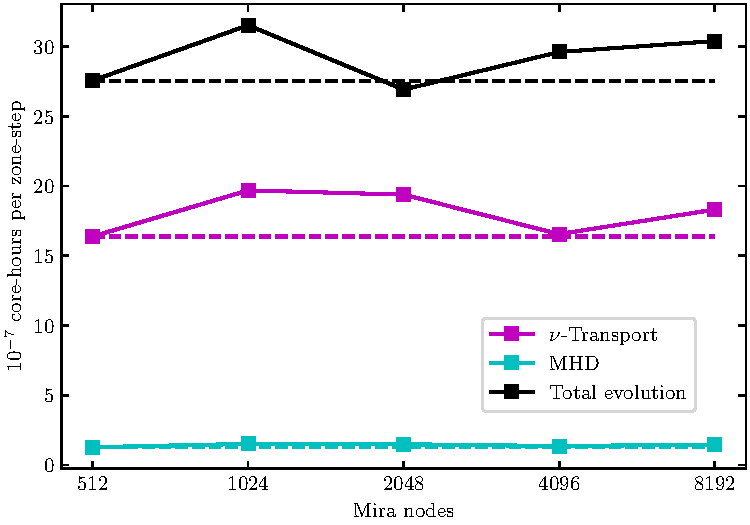
\includegraphics[width=3.2in]{figs/wkScaleSparkM1} \\
    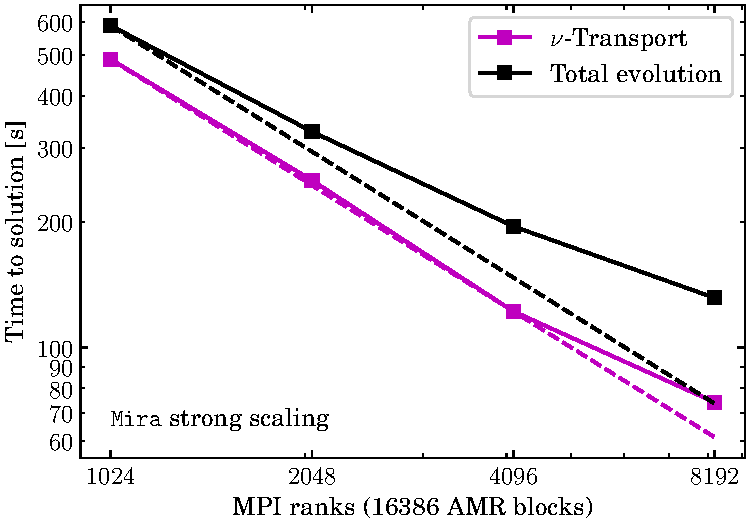
\includegraphics[width=3.2in]{figs/strScaleSparkM1} \\
    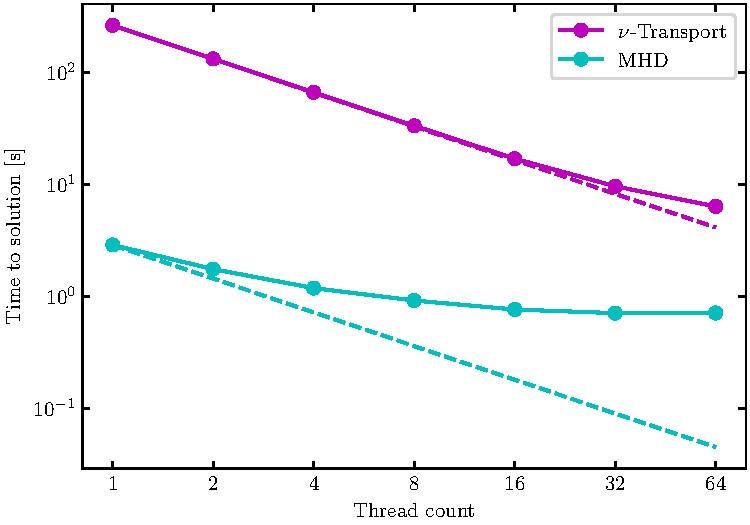
\includegraphics[width=3.2in]{figs/thrdSpeedupSparkM1}
  \end{tabular}
  \caption{Weak scaling (top), strong scaling (middle), and threading
  speedup (bottom) of \sparkmone on {\it Mira}.}
  \label{fig:scaling}
%\end{figure}
\end{wrapfigure}
FLASH contains a wide range of numeric solvers for solving
PDEs on block-structured AMR meshes. FLASH relies on the oct-tree
based PARAMESH library \citep{MacNeice:2000}. The proposed
simulations will solve the equations of hydrodynamics and
magnetohydrodynamics using an unsplit, explicit, finite-volume
Eulerian formulation (see Sec. \ref{sec:spark}).
FLASH utilizes hybrid MPI/OpenMP parallelism in order to make best use
of many-core architectures. The hydrodynamics/MHD
solvers, gravity solvers, and source terms have all been extended to
include support for thread-level parallelism via OpenMP.
FLASH writes output files using the HDF5 library. These files can be
read in directly and visualized in parallel using VisIt or yt
visualization software \citep{Turk:2011}.


Our \sparkmone application has been architected for performance.
Options such as reconstruction and Riemann solver are selected at compilation rather than runtime and are generally directly in-lined into the  calling routines in order to avoid function call overhead.
Aggressive use of Fortran array operations are employed and facilitate easy vectorization by the compiler.
In order to minimize cache misses, the reconstruction and flux calculation steps in \spark take place on auxiliary 1D ``pencil'' arrays that flatten an entire 1D ray of zones into a data structure that is contiguous in memory and much smaller than a one entire AMR block data structure.
All 1D reconstruction and flux computations are completed on these rays then before moving on to other rays, maximizing the number of operations performed per byte of data moved from memory.
This approach also facilitates efficient OpenMP threading wherein each thread operates on a collection of pencil arrays.
Communication is avoided during the multi-stage RK integration by filling and updating extra layers of guard, or halo, zones.
Thus, for WENO5, with a five-point stencil, and RK2 we require six guard zones per direction.
The M1 neutrino transport equations form a hyperbolic system of PDEs that is extremely similar to the MHD equations in structure and, thus, can be solved with similar methods.
Our implementation is a finite volume approach using second-order spatial reconstruction and third-order SSP RK time integration.
This approach makes full use of all six guard zones per direction and the high-order time integration increases stability, allowing M1-limited time steps up to CFL factors of $\gtrsim$0.9, greater than the typical MHD-limited CFL factor of $\sim$0.5.
This mitigates to some extent the increased number of time steps required by the explicit radiation transport approach and reduces the ratio of communication-to-calculation.


\subsubsection{Workflow Patterns}
\label{sec:workflow}

Our proposed research plan involves a multitude of simulations almost of all of which require several restarts and extensive post-processing visualization and analysis.
In the past, we have used the Simulation management and analysis
system (Smaash) that was custom-built for FLASH simulations.
We found Smaash to have some nice features, but to suffer from portability and stability and have since resorted to shell scripts for automatically configuring and queuing restart jobs.
This approach is robust and portable, but lacks any degree of in-flight monitoring, analysis, or visualization and is generally still very ``hands-on.''
We are currently developing a new simulation management tool in Python that seeks to retain the simplicity and portability of our shell scripts while being more full-featured.
This management tool, \SIMpliPy, will monitor simulation progress and perform simple runtime analysis and visualization using yt \citep{Turk:2011}.
\SIMpliPy will also configure and schedule job restarts, handle job dependencies, and manage automatic transferal of simulation data to archival storage.
\SIMpliPy is borrowing ideas and features from the {\tt sumatra} tool \footnote{https://pythonhosted.org/Sumatra/} to enhance reproducibility of simulations and data provenance.
\SIMpliPy will primarily use standard Python features and libraries (such as JSON for metadata management) and git for version tracking in order to both speed development and provide portability.



\subsubsection{I/O}

Flash implements parallel HDF5 and collective I/O wherein a reduced
number of MPI ranks perform I/O to reduce the number of processes
accessing the file system at one time. The amount of time spent by
FLASH on I/O in a production simulation is typically less than 10\% of the overall run time.



\begin{figure}
  \begin{tabular}{ll}
    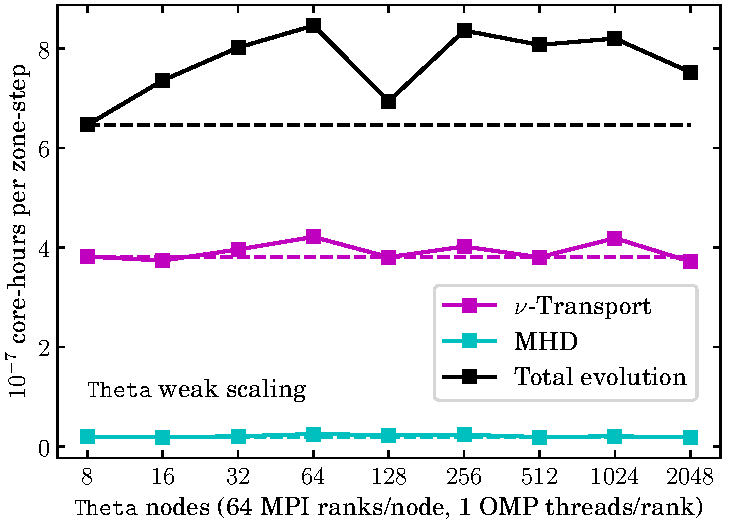
\includegraphics[width=3.2in]{figs/wkScaleSparkM1_theta} & \hspace{-16pt}
    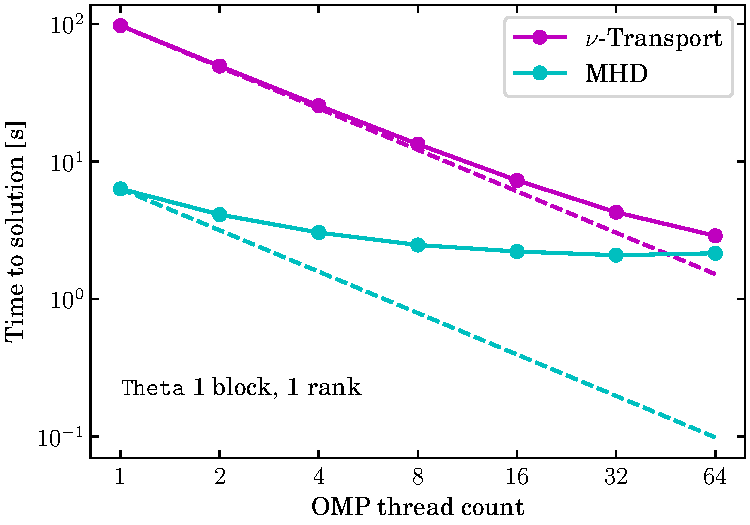
\includegraphics[width=3.2in]{figs/thrdSpeedupSparkM1_theta}
  \end{tabular}
  \caption{Weak scaling (left) and OpenMP thread-to-thread speedup for our \sparkmone CCSN application on \thet.}
  \label{fig:thetaScaling}
\end{figure}


\subsection{Parallel Performance}
\label{sec:performance}


We have benchmarked the performance and scaling of our \sparkmone application on \mira, \thet, as well as commodity computers using recent Intel processors.
Our scaling studies use the full, production version of \sparkmone, including MHD, self-gravity, AMR, M1 neutrino transport, and tabular equation of state.
In Figure \ref{fig:scaling} we show the weak scaling on {\it Mira} for \sparkmone going up to the entire machine, 49,152 nodes (786k cores).
Weak scaling is essentially perfect, with an efficiency of 92\% at 48,152 nodes as compared to 512 nodes, with some scatter as these tests represent realistic production-grade problem setups.
This result is a dramatic improvement in weak scaling efficiency for our M1 neutrino transport application as compared to our INCTE proposal in 2014.
We also plot in Fig. \ref{fig:scaling} the strong scaling and thread-to-thread speedup for \sparkmone.
Our production simulations as planned will typically have four or more AMR blocks per MPI rank, putting them not near to the ideal strong scaling curve.
OpenMP thread speed up is near-perfect for the M1 solver, although cache contention at more than 16 threads per rank becomes an issue).
Threading efficiency could be improved for our MHD solver, but it typically represents a small fraction of overall runtime for our planned simulations and so is not a limiting factor.

We have also carried out an initial performance study of our \sparkmone application on \thet.
Figure \ref{fig:thetaScaling} shows the weak scaling and threading speedup on \thet.
Both are acceptable for our planned production simulations on \thet, but we stress that this is only on initial performance study as we have not yet done any performance tuning of \sparkmone on \thet, only ported our application directly from \mira.
Thus, we expect to realize substantial improvements in performance on \thet although we are already seeing an increase in per-core performance of 4x over \mira for \sparkmone!
This is better even than the nominal increase in per-core FLOP rate between these two machines (3.25x).

In order to gauge the absolute performance of our new \spark MHD solver, we have benchmarked \spark against \flash's unsplit staggered-mesh constrained transport solver (USM-CT).
We use the common Field Loop Advection problem described in \citet{Gardiner:2005} and \citet{Lee:2009}, which is a standard test problem packaged with the release versions of both codes.
We have executed this benchmark on four different hardware platforms: a commodity laptop with a Intel Core i7 6567U processor, a Lenovo cluster with Intel Xeon E5-2680v4 processors, BG/Q {\tt Cetus} with IBM A2 processors, and \thet with Intel Phi-Knights Hill chips.
We use a fixed-resolution grid for these tests and the same parameters on all platforms using a single thread of execution.

The results of this benchmarking are shown in Table \ref{table:perf}.
On all platforms, \spark outperforms the USM-CT solver by a factor of $\sim$3-4.
Table \ref{table:perf} also shows the single-thread performance for our \sparkmone CCSN application on these hardware platforms.
Most notable is the increase in performance between BG/Q and Intel KNL.
Without yet having done {\it any} machine-specific tuning for \thet, we find an increase in single-thread performance of $\sim$4x over IBM BG/Q.
The numbers for \sparkmone in this table are used in making the required resource estimates throughout this proposal.



\begin{deluxetable}{lllll}
\tablecolumns{5}
\tabletypesize{\scriptsize}
\tablecaption{
Single-thread performance comparisons on different hardware platforms in units of core-hours/zone-step (zone-step/core-second).
\label{table:perf}
}
\tablewidth{0pt}
\tablehead{
\colhead{ } &
\colhead{FieldLoop \spark} &
\colhead{FieldLoop USM-CT} &
\colhead{CCSN \sparkmone} &
\colhead{Progen {\tt Spark-Ap21}}
}
\startdata
  Intel Core i7 (I7-6567U) & 2.15e-09 (129,075) & 7.09e-09 (39,173) & 1.80e-07 (1545) & 4.30e-09 (64,378) \\
  Intel Xeon E5-2680v4     & 1.76e-09 (157,808) & 4.42e-09 (62,779) & 1.05e-07 (2658) & 3.52e-09 (78,904)\\
  IBM BG/Q A2              & 2.58e-08 (10,787)  & 6.58e-08 (4221)   & 2.75e-06 (103) & 5.16e-08 (5393) \\
  Intel KNL                & 7.41e-09 (37,494)  & 2.81e-08 (9881)   & 7.00e-07 (397) & 1.48e-08 (18,747)
\enddata
\end{deluxetable}


\subsection{Developmental Work}

Our \sparkmone application is production ready for the simulations we plan for Year 1 of this project.
During Year 1, we will profile and tune \sparkmone on \thet.
We also plan to implement a ``marching cubes'' scheme for storing EOS and opacity data.
In this approach, only the portion of the very large ($\sim$400 MB each) tables that is needed by a given MPI rank will be stored in that rank's memory. Ideally, this would make the EOS and opacity data fit within the outer-most level of cache enabling substantial increase in performance.
On \thet, this approach will ensure that the entire application easily fits within the high-bandwidth memory.
One of the project postdocs, Kuo-Chuan Pan, is attending the Argonne Training Program in Extreme-Scale Computing and will focus on tuning our application for \thet.

Much of the remainder of our development plans are targeted toward next-generation systems such as \aurora (see following section).


\subsection{Development plan for next-generation systems}

% Our application, like many physics applications, is memory bandwidth-bound.
% As such, we aim to utilize almost exclusively the high-bandwidth on-package memory of the Intel Knights (Landing/Hill) architecture for the actual compute side of our application.
% In order to achieve good performance and scaling on this type of platform, we plan to implement MHD and radiation transport algorithms with high arithmetic intensities.
We will implement very high-order cell-centered constrained transport finite difference MHD methods \citep{Christlieb:2014, Christlieb:2016}.
Using the method of differential transforms \citep{Norman:2012, Norman:2013, Seal:2014a}, we will achieve not only high spatial order but high temporal order as well while maintaining a very compact spatial stencil, thus limiting the need for large numbers of ghost zones and attendant (expensive) inter-node communication.
For example, a ninth-order WENO method using the method of differential transforms requires only eleven ghost zones per dimension to achieve ninth-order temporal accuracy \citep{Seal:2014a}.
% Both spatial {\it and} temporal accuracy are critical to accurately modeling turbulence.
Additionally, we explore implementing order-adaptivity such that the spatial and temporal orders will be decreased in, e.g., shocks where high-order finite difference is undesirable.

% In addition to implementing new high-order finite difference algorithms for MHD, we will re-architect the loop structure of the MHD solver to better utilize cache and reduce memory movement.
% Our approach for this will be to compute all the 1D fluxes for a given dimension in a single pass before moving on to the other dimensions.
% By using auxiliary 1D arrays into which the contiguous data along a given ray is temporarily copied, the entire stencil on which the solution depends can be easily fit into cache and made genuinely local in the memory address space (i.e., all stride-one).
% This approach also makes threading the calculation straightforward and efficient.
% For example, for a domain of size $64^3$ there would be $64^2$ ``rays'' in a given direction each of length $64$.  The computation of the 1D fluxes on these rays is completely independent of the data on the rays, making parallelization via threads trivial.
% Additionally, since many of the operations involved in the flux calculation must be done on multiple variables independently, vectorizations of the calculation is easy and efficient.

% We have already implemented a prototype hydrodynamics solver in \flash using the approach described in the previous paragraph.
% This prototype solver uses third-order spatial reconstruction and second-order Runge-Kutta temporal integration in the method-of-lines approach.
% All else being equal, the single-core performance of this prototype is fully {\it twice} that of the current directionally unsplit hydro solver available in \flash \citep{Lee:2013}.
% This prototype will serve as the framework in which we implement very high-order finite difference MHD methods for use in this project.

We will also overhaul the main driver routines in \flash to incorporate some limited task-based parallelism and one-sided MPI communication.
For the former, we will use the unique \flash build system to define {\tt TASKS} and respective {\tt DEPENDENCIES}.
Physics solvers such as MHD are stencil based and thus have some dependence on neighboring data requiring that these operations wait until the ghost zone data are received from neighboring processes.
Other solvers, such as nuclear burning and other local source terms, are not stencil based and so can be completed before ghost zone data are received.
By restructuring the top-level driver routine in \flash, we will exploit these differences in dependencies to increase the parallel efficiency of the application using a very limited form of task-based parallelism.
This approach can even be extended to stencil-based operators such as MHD by taking advantage of the fact that the stencils used are typically much smaller than the linear size of the domain blocks, the fundamental units of parallelism in \flash.
Thus the domain blocks can be further sub-divided into completely node-local ``tiles.''
Some tiles will not have stencils that extend into any ghost zone regions and can therefore be computed before waiting for ghost zone communication to complete.
Other tiles will depend on ghost zone data from a subset of the neighboring processes and can then be worked on once communication is completed with only those processes.

We also plan to overhaul the ghost zone communication in \flash by incorporating one-sided MPI communication through the use of user buffers for storing messages.
These buffers may be in the NVRAM or the DDR4, while the memory needed by the task currently being executed will sit in the HBM.

% We also aim to take full advantage of the novel NVRAM planned for \aurora.
% We plan to implement an on-the-fly ``flash'' checkpointing method that will store several copies of the previous solution state every few time steps in the NVRAM.
% These stored copies of the previous solutions can be used in several ways.
% First, using machine learning, these data could be used to adaptively and intelligently decide when a checkpoint should be written to disk.
% I.e., the machine learning would detect when ``something interesting'' was happening in the data and then signal the application to write the data to disk for analysis.
% The flash checkpoints could also be used for doing {\it in-situ} analysis on the data stored in the NVRAM, allowing a broad range of time dependent analysis that need good temporal resolution without any need to write the full data out to disk.
% Another nice feature of this approach is the possibility for fault-tolerance.
% If the checkpoints stored in the NVRAM were to be setup in a RAID-like data striping configuration amongst a subset of spatially co-located nodes, if one of these node were to experience a fault or complete failure, the data from the most recent checkpoint could be completely reconstructed.
% The simulation could then proceed without a complete failure by either making a prediction of the state of the lost data at the current simulation time or by re-evolving the solution from this last saved checkpoint.


% For I/O we will continue to rely on the HDF5 library.
% We will engage with the ExaHDF5 team to get early access to new features designed and optimized for \aurora's architecture.
% We will also seek to collaborate with the ExaHDF5 team on incorporate some of the features we suggest here such as flash checkpointing and NVRAM data striping into the HDF5 library, as appropriate.
% Features similar to these may already be planned for HDF5 making extension to the application use we plan here straightforward.
% We also intend to rely on extensions to the HDF5 library to allow our \flash application to take advantage of novel features of \aurora such as I/O burst buffers.

We will also explore the possibility of implementing a novel data compression algorithm for time-series physics simulation data.
For physics simulations that include small scale features that are {\it not} volume-filling, the full domain data does not need to be written to disk as frequently as regions that contain features of interest.
This presents the opportunity for dramatic data compression through implementing an I/O scheme that adaptively selects subsets of the full domain data to write to disk frequently.
For post-processing analysis and visualization could then be achieved by using image reconstruction methods to recover the coarsely sampled data at the desired sampling frequency.
Machine learning methods could be employed to intelligently save data at the correct sampling rate to retain a specified level of accuracy in the reconstructed data.
We will engage the ExaHDF5 group in the feasibility of implementing such an I/O scheme.

Our approach for portability in this project will be to continue \flash's reliance principally on MPI and HDF5 while incorporating the emerging OpenMP 4.x standard for on-node thread parallelism.
OpenMP 4.x implements unified directives for both many-core chips such as Intel Phi and for GPGPU accelerators.
The physics solvers in \flash are already threaded using OpenMP so the extension to the new 4.x standard will be relatively straightforward.

% The application development proposed as part of this project will focus on uniform grid applications, avoiding the need to adapt \flash's current AMR grid package to \aurora.
% A number of other initiatives are underway to incorporate new AMR grid packages into \flash, specifically BoxLib and Cello.
% Several of the PI's of this ESP project are directly involved in these efforts.
% Our work in adapting \flash's physics solvers to \aurora and other pre-exascale platforms will be done in close coordination with the efforts to implement new AMR grid packages and parallelism to \flash, maximizing the impact of all of these projects.
